% 2015-05-21 - Emerson Ribeiro de Mello - mello@ifsc.edu.br
% \documentclass[handout,xcolor=pdftex,dvipsnames,table]{beamer}
\documentclass{beamer}

\usepackage[utf8]{inputenc}
\usepackage[T1]{fontenc}
\usepackage[english,brazil]{babel}
\let\sup\textsuperscript
\let\subs\textsubscript
% \setbeameroption{show notes on second screen=right}


% usando tema personalizado. 
% arquivo beamerthemeIFSC.sty deve estar no mesmo diretório do .tex
\usepackage{beamerthemeIFSC}


\hypersetup{pdfstartview={Fit},pdftitle={\@title},
 	pdfsubject={Engenharia de Telecomunicacoes - IFSC},pdfauthor={\@author}
}



%%%%%%%%%%%%%%%%%%%%%%%%%%%%%%%%%%%%%%%%%%%%

\newcommand{\DAY}{\the\day}
\newcommand{\MONTH}{%
    \ifcase\the\month
    \or Janeiro%
    \or Fevereiro%
    \or Março%
    \or Abril%
    \or Maio%
    \or Junho%
    \or Julho%
    \or Agosto%
    \or Setembro%
    \or Outubro%
    \or Novembro%
    \or Dezembro%
    \fi}
\newcommand{\YEAR}{\the\year}

\title{EDB18802 - Eletrônica Digital II:}
\subtitle{\LARGE Latches SR e D}
\author{João Cláudio Elsen Barcellos}
\date{\scriptsize \DAY~de \MONTH~de \YEAR}
\institute{Engenheiro Eletricista\\
Formado na Universidade Federal de Santa Catarina\\
campus Florianópolis\\
\url{joaoclaudiobarcellos@gmail.com}
}



%%%%%%%%%%%%%%%%%%%%%%%%%%%%%%%%%%%%%%%%%%%%

\begin{document}

\captionsetup{labelformat=empty}

\begin{frame}[t]
    % Example of a note:
    % \note{Boa tarde a todos, na aula de hoje iremos estudar os circuitos sequenciais...}
    \maketitle
    \vspace{-1cm}
    \begin{flushleft}
        \vfill
        \textit{\tiny $^{*}$Créditos ao Prof. Emerson Ribeiro de Mello, o qual criou e disponibilizou o template aqui usado, via ShareLaTeX}\par
    \end{flushleft}
\end{frame}

% Descomente as linhas abaixo se desejar colocar um sumário de todas as seções
\begin{frame}[t]{Plano de aula}
    \tableofcontents

    % Notas
    % \note{...E, para isso, organizei o conteúdo da seguinte forma: começaremos com uma introdução ao tema, comparando os circuitos combinacionais e sequenciais. Em seguida, apresentarei o principal componente de um circuito sequencial: o elemento de memória. Nesse contexto, estudaremos os latches (dos tipos SR e D) e os flip-flops (do tipo D). Depois, demonstrarei uma simulação no software ISE, que poderá ser utilizado ao longo do semestre para auxiliar na compreensão do funcionamento de circuitos digitais. Na simulação de hoje, trabalharemos com um flip-flop do tipo D. Por fim, ao término da aula, disponibilizarei algumas referências e sugestões de leitura complementar.}
\end{frame}


\def\sectionname{}
\def\insertsectionnumber{}
\def\subsectionname{}
\def\insertsubsectionnumber{}

\AtBeginSection{\frame{\sectionpage}\addtocounter{framenumber}{-1}}


\AtBeginSubsection{\frame{\subsectionpage}\addtocounter{framenumber}{-1} }
\AtBeginSubsubsection{\frame{\subsubsectionpage}\addtocounter{framenumber}{-1} }






%%%%%%%%%%%%%%%%%%%%%%%%%%%%%%%%%%%%%%%%%%%%
% Inicio do documento
%%%%%%%%%%%%%%%%%%%%%%%%%%%%%%%%%%%%%%%%%%%%


\section{Introdução}

\begin{frame}
    \frametitle{\insertsection}
    \begin{columns}
        \scriptsize

        \begin{column}[t]{0.3\textwidth}
            \vbox{
                \centering
                \begin{itemize}
                    \item Circuitos digitais nos quais a saída depende exclusivamente do estado atual de suas entradas são classificados como: \textbf{circuitos combinacionais};
                    \item Não possuem memória, ou seja, não armazenam informações quanto à estados anteriores;
                    \item Alguns exemplos são: multiplexador, comparador, decodificador, unidade lógica e aritmética (para operações matemáticas e lógicas).
                \end{itemize}
            }
        \end{column}
        
        \begin{column}[t]{0.3\textwidth}
            \vbox{
                \centering
                \captionof{figure}{}
                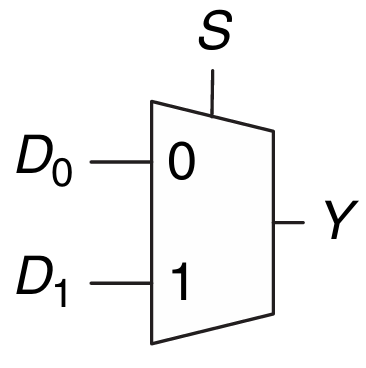
\includegraphics[width=0.4\columnwidth]{figures/mux.png}
                \caption*{\tiny Fonte: HARRIS; HARRIS (2015)}
                  
                \captionof{figure}{}
                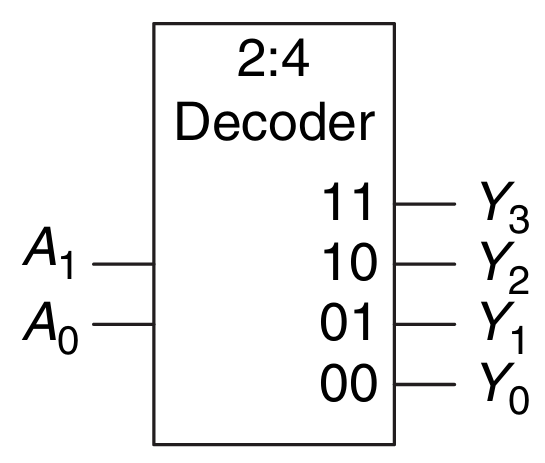
\includegraphics[width=0.4\columnwidth]{figures/decoder.png}
                \caption*{\tiny Fonte: HARRIS; HARRIS (2015)}
            }
        \end{column}
        
        \begin{column}[t]{0.3\textwidth}
            \vbox{
                \centering
                \captionof{figure}{}
                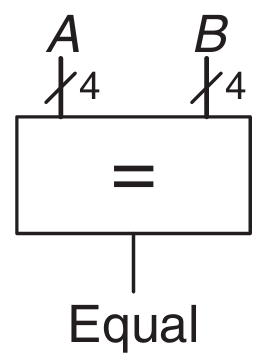
\includegraphics[width=0.3\columnwidth]{figures/comparator.png}
                \caption*{\tiny Fonte: HARRIS; HARRIS (2015)}
                
                \captionof{figure}{}
                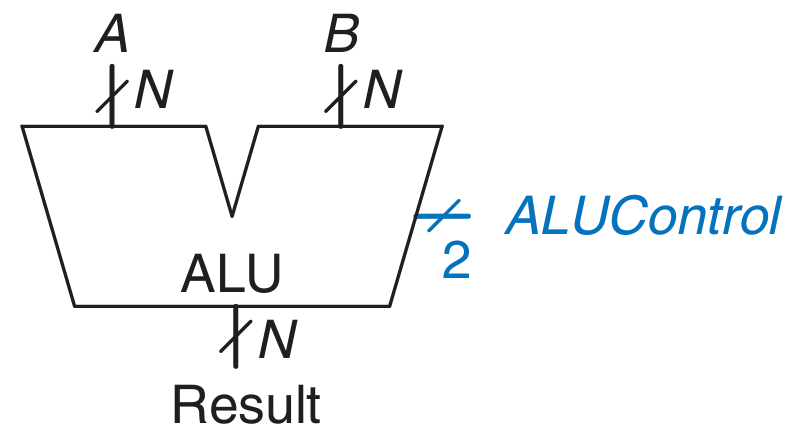
\includegraphics[width=0.6\columnwidth]{figures/alu.png}
                \caption*{\tiny Fonte: HARRIS; HARRIS (2015)}
            }
        \end{column}    
        
    \end{columns}

    % Notas
    % \note{Bom, vamos começar falando dos circuitos combinacionais. Esses são os circuitos cuja saída depende apenas do estado atual de suas entradas, sem envolver nenhum elemento de memória. Por isso, eles não conseguem armazenar os estados das entradas ou saídas. Exemplos comuns de circuitos combinacionais incluem portas lógicas, somadores e multiplexadores. Então, a principal característica desses circuitos é que a saída é sempre uma função direta das entradas, sem nenhuma relação com estados anteriores.}
\end{frame}

\begin{frame}
    \frametitle{\insertsection}

    \begin{columns}
        \scriptsize

        \begin{column}[t]{0.3\textwidth}
            \vbox{
                \centering
                \begin{itemize}
                    \item Circuitos digitais nos quais a saída depende não só do estado atual de suas entradas, mas também de estados anteriores são classificados como: \textbf{circuitos combinacionais};
                    \item Possuem memória, ou seja, são capazes de reter informações quanto a estados anteriores;
                    \item Alguns exemplos são: contador, máquina de estados finitos.
                \end{itemize}
            }
        \end{column}
        
        \begin{column}[t]{0.65\textwidth}
            \vbox{
                \centering
                \captionof{figure}{}
                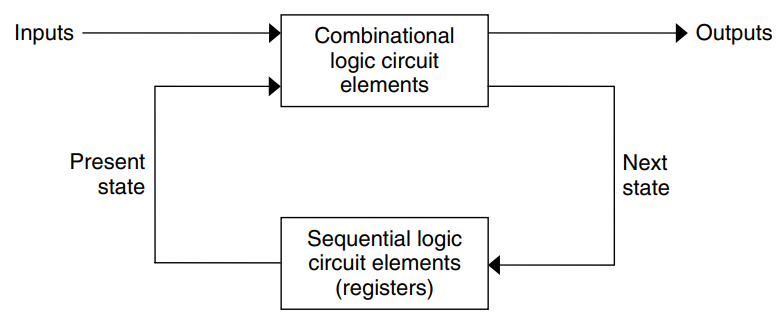
\includegraphics[width=\columnwidth]{figures/sequential_circuit.png}
                \caption*{\tiny Fonte: GROUT (2008, p. 278)}
            }
        \end{column}   
        
    \end{columns}
    
    % Notas
    % \note{Agora, falando dos circuitos sequenciais, eles são baseados em elementos de lógica combinacional (como portas AND, OR, entre outras) trabalhando em conjunto com elementos de memória, como latches e flip-flops (que, juntos, podem formar registradores). Nesse caso, a saída não depende apenas das entradas atuais, mas também de estados anteriores. Alguns exemplos de circuitos sequenciais são os contadores, registradores e máquinas de estados.}
\end{frame}

\section{Latches}

\begin{frame}
    \frametitle{\insertsection}
    \begin{columns}
        \scriptsize
        \begin{column}[t]{0.45\textwidth}
            \vbox{
                \centering
                \begin{itemize}
                    \item Latches são usados para armazenar um único bit de informação;
                    \item O Latch é um circuito biestável, o que significa que ele pode estar em um de dois estados estáveis: 0 ou 1;
                    \item Latches são formados por portas lógicas (como NOR ou NAND) e possuem entradas de controle para definir ou alterar seu estado;
                    \item São elementos de memória mais ``básicos''.
                \end{itemize}

            }
        \end{column}
        
        \begin{column}[t]{0.45\textwidth}
            \vbox{
                \centering
                \captionof{figure}{}
                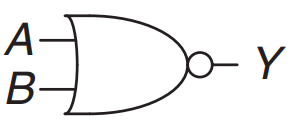
\includegraphics[width=0.6\columnwidth]{figures/nor.png}
                \caption*{\tiny Fonte: HARRIS; HARRIS (2015, p. 21)}

                \begin{tabular}{cc|cc}
                    A & B & Y \\
                    \hline
                    & &\\
                    0 & 0 & 1 \\
                    0 & 1 & 0 \\
                    1 & 0 & 0 \\
                    1 & 1 & 0 \\
                \end{tabular}
            }
        \end{column}    
    \end{columns}

        % Notas
    % \note{Latches são elementos de memória capazes de armazenar informações de até um bit. Além disso, são considerados biestáveis, o que significa que possuem dois estados que são estáveis: 0 ou 1. São elementos de memória bastante ``básicos'', já que são formados por portas lógicas, como NORs e NANDs. Inclusive, a sua forma mais ``básica'' é o dito latch SR, o qual será visto a seguir. Para isso, iremos utilizar portas NOR para montá-lo e analizá-lo. Ao lado, apenas para recapitular, há uma NOR, com sua tabela verdade. Percebamos que a única situação na qual sua saída será igual a 1 é quando ambas as entradas, A e B, são iguais a 0. Dessa forma, se uma de suas entradas for igual a 1, isso já é suficiente para que sua saída seja igual a 0.}
    
\end{frame}

\subsection{Latch SR (\textit{set-reset})}

\begin{frame}
    \frametitle{\insertsubsection}
    \begin{columns}
        \scriptsize
        \begin{column}[t]{0.4\textwidth}
            \vbox{
                \centering
                \captionof{figure}{}
                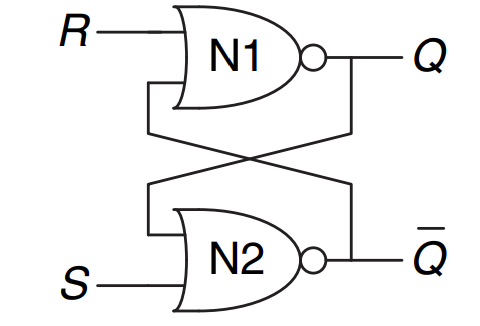
\includegraphics[width=0.6\columnwidth]{figures/latch_sr_schematic.png}
                \caption*{\tiny Fonte: HARRIS; HARRIS (2015)}
                
                \vspace{-0.1cm} % Espaço negativo para reduzir a distância entre as figuras
                

            }
        \end{column}
        
        \begin{column}[t]{0.5\textwidth}
            \vbox{
                \centering
                \captionof{figure}{}
                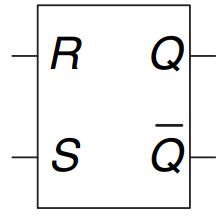
\includegraphics[width=0.4\columnwidth]{figures/latch_sr_symbol.png}
                \caption*{\tiny Fonte: HARRIS; HARRIS (2015)}
                
                \vspace{-0.1cm} % Espaço negativo para reduzir a distância entre as figuras
                

            }
        \end{column}    
    \end{columns}
    \begin{center}
        \begin{tabular}{cc|cc}
            R (``resetar'') & S (``setar'') & Q (saída) & \=Q (complemento da saída) \\
            \hline
            & & &\\
            0 & 0 & Q\subs{anterior} & \=Q\subs{anterior}\\
            0 & 1 & 1 & 0 \\
            1 & 0 & 0 & 1 \\
            \textcolor{red}{1} & \textcolor{red}{1} & \textcolor{red}{invalido} & \textcolor{red}{invalido} \\
        \end{tabular}
    \end{center}
\end{frame}

\begin{frame}
    \frametitle{\insertsubsection}
    \begin{columns}
        \scriptsize
        
        \begin{column}[t]{0.45\textwidth}
            \vbox{
                \centering
                \captionof{figure}{}
                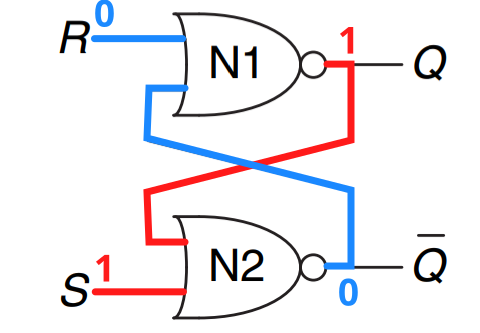
\includegraphics[width=0.5\columnwidth]{figures/latch_sr_set.png}
                \caption*{\tiny Fonte: modificado de HARRIS; HARRIS (2015)}
                  
                \captionof{figure}{}
                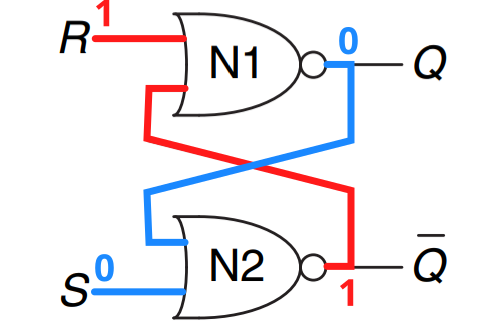
\includegraphics[width=0.5\columnwidth]{figures/latch_sr_reset.png}
                \caption*{\tiny Fonte: modificado de HARRIS; HARRIS (2015)}
            }
        \end{column}
        
        \begin{column}[t]{0.45\textwidth}
            \vbox{
                \centering
                \captionof{figure}{}
                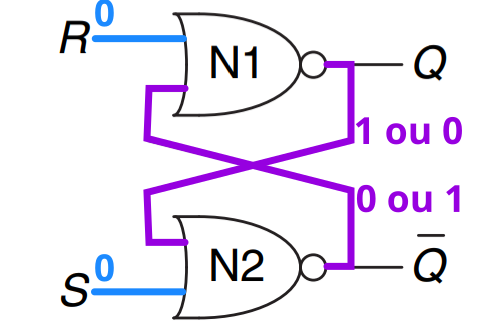
\includegraphics[width=0.5\columnwidth]{figures/latch_sr_wait.png}
                \caption*{\tiny Fonte: modificado de HARRIS; HARRIS (2015)}
                
                \captionof{figure}{}
                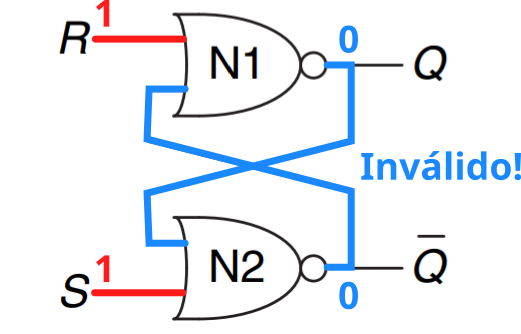
\includegraphics[width=0.5\columnwidth]{figures/latch_sr_invalid.png}
                \caption*{\tiny Fonte: modificado de HARRIS; HARRIS (2015)}
            }
        \end{column}    
        
    \end{columns}
\end{frame}

\subsection{Latch D}

\begin{frame}
    \frametitle{\insertsubsection}
    \begin{columns}
        \scriptsize
        \begin{column}[t]{0.4\textwidth}
            \vbox{
                \centering
                \captionof{figure}{}
                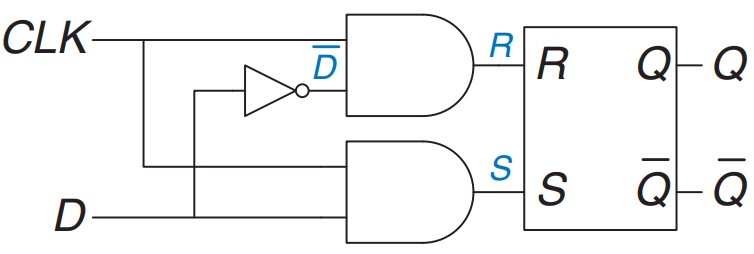
\includegraphics[width=\columnwidth]{figures/latch_d_schematic.png}
                \caption*{\tiny Fonte: HARRIS; HARRIS (2015)}
                
                \vspace{-0.1cm} % Espaço negativo para reduzir a distância entre as figuras
            }
        \end{column}
        
        \begin{column}[t]{0.5\textwidth}
            \vbox{
                \centering
                \captionof{figure}{}
                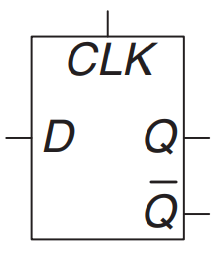
\includegraphics[width=0.4\columnwidth]{figures/latch_d_symbol.png}
                \caption*{\tiny Fonte: HARRIS; HARRIS (2015)}
                
                \vspace{-0.1cm} % Espaço negativo para reduzir a distância entre as figuras
            }
        \end{column}    
    \end{columns}
    \begin{center}
        \begin{tabular}{cc|ccc|cc}
            CLK & D & \=D & R (``reset'') & S (``set'') & Q (saída) & \=Q (compl. da saída) \\
            \hline
            & & & & & &\\
            0 & X & \=X & 0 & 0 & Q\subs{anterior} & \=Q\subs{anterior}\\
            1 & 0 & 1 & 0 & 1 & 0 & 1 \\
            1 & 1 & 0 & 1 & 0 & 1 & 0 \\
        \end{tabular}
    \end{center}
\end{frame}

\begin{frame}
    \frametitle{\insertsubsection}
    \begin{columns}
        \scriptsize
        \begin{column}[t]{0.45\textwidth}
            \vbox{
                \centering
                \captionof{figure}{}
                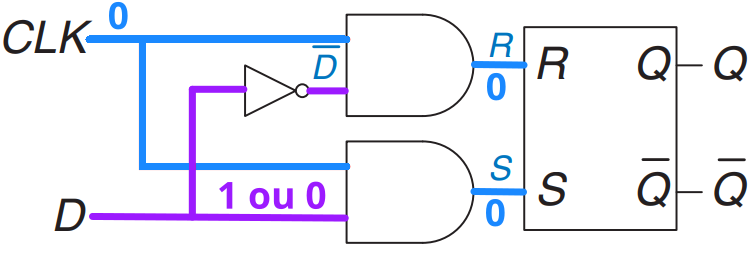
\includegraphics[width=\columnwidth]{figures/latch_d_clock_low.png}
                \caption*{\tiny Fonte: modificado de HARRIS; HARRIS (2015)}
                
                \vspace{-0.1cm} % Espaço negativo para reduzir a distância entre as figuras
            }
        \end{column}
        
        \begin{column}[t]{0.45\textwidth}
            \vbox{
                \centering
                \captionof{figure}{}
                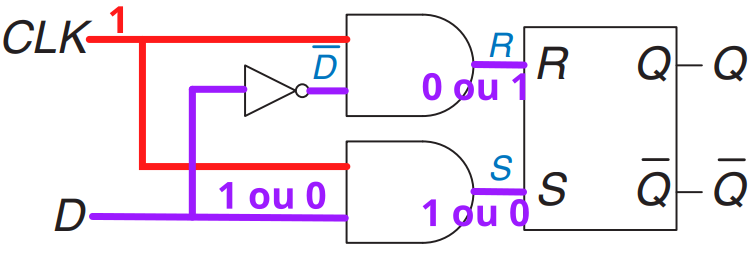
\includegraphics[width=\columnwidth]{figures/latch_d_clock_high.png}
                \caption*{\tiny Fonte: modificado de HARRIS; HARRIS (2015)}
                
                \vspace{-0.1cm} % Espaço negativo para reduzir a distância entre as figuras
            }
        \end{column}    
    \end{columns}
\end{frame}


\section{Simulação no Logisim}

\begin{frame}
    \frametitle{\insertsection}
    \centering
    
\includegraphics[width=0.15\columnwidth]{figures/Logo_Logisim.png}
    
    \vspace{1em}
    
    \begin{itemize}
        \item Para consolidar os conceitos apresentados em aula, realizamos a simulação de dois circuitos utilizando o Logisim:
        \begin{itemize}
            \item Um \textbf{Latch} implementado com lógica combinacional;
            \item Um \textbf{Latch do tipo D}, utilizado para armazenar um bit de forma controlada.
        \end{itemize}
        \item A simulação permite observar o comportamento dos circuitos frente às variações nas entradas de controle e dados.
        \item É possível analisar a diferença entre os dois dispositivos em termos de sensibilidade ao clock e resposta às entradas.
    \end{itemize}
\end{frame}


\section{Conceitos para a próxima Aula}

\begin{frame}
    \frametitle{Latch D vs Flip-Flop D}

    \begin{table}[h!]
    \centering
    \scalebox{0.73}{ % ajuste a escala aqui (ex: 0.8, 1.0, 1.2 etc)
    \begin{tabular}{|l|c|c|}
    \hline
    \textbf{Característica} & \textbf{Latch D} & \textbf{Flip-Flop D} \\
    \hline
    Tipo de ativação & Nível sensível (Level-triggered) & Borda sensível (Edge-triggered) \\
    \hline
    Atualização & Enquanto o clock (ou enable) estiver ativo & Apenas na transição (borda) do clock \\
    \hline
    Complexidade & Mais simples & Mais estável para contadores \\
    \hline
    Uso típico & Armazenamento temporário & Circuitos sequenciais \\
    \hline
    \end{tabular}
    } % fim do scalebox
    \caption{Comparação entre Latch D e Flip-Flop D}
    \label{tab:comparacao_latch_flipflop}
    \end{table}
\end{frame}


\begin{frame}
    \frametitle{Próxima Aula: Introdução aos Flip-Flops}

    \begin{itemize}
        \item Vamos iniciar o estudo dos \textbf{Flip-Flops}.
        \item Flip-Flops são \textbf{elementos de memória síncronos}, sensíveis à borda do clock.
        \item Eles serão amplamente utilizados ao longo do semestre para:
        \begin{itemize}
            \item Construção de contadores.
            \item Implementação de registradores.
            \item Projetos de máquinas de estados.
        \end{itemize}
        \item Compreender os Flip-Flops é essencial para o desenvolvimento de circuitos sequenciais.
        \item A base para muitos dos projetos digitais que faremos será formada a partir deles.
    \end{itemize}

    \vspace{0.5cm}

  
\end{frame}



\section{Referências e sugestões de leitura}
\begin{frame}
    \frametitle{\insertsection}
    \begin{enumerate}
        \item SILVINA HANONO WACHMAN. MIT 6.004 L06: Sequential Circuits. Disponível em: <https://www.youtube.com/watch?v=hf0g3Ccfer8>. Acesso em: 25 nov. 2024.
        \item GHOSH, B. Basics of Digital Electronics. [s.l.] CRC Press, 2023.
        \item HARRIS, S. L.; DAVID MONEY HARRIS. Digital design and computer architecture. Amsterdam ; Paris: Elsevier, Cop, 2015.
        \item GROUT, I. Digital Systems Design with FPGAs and CPLDs. Burlington: Elsevier, 2008.
    \end{enumerate}
\end{frame}

\end{document}